\chapter{Deep Learning}\label{chapter:deeplearning}
Machine Learning in recent time runs in the heart of every artificially intelligent system, from image and text search on the web, to recommendation systems in popular e-commerce websites, to automatic tagging of your photos on social networking sites etc. Machine Learning has allowed us to create some very interesting applications which were not possible few decades ago. A prominent requirement in traditional machine learning systems is the use of hand labeled tagged data-set for a specific task, upon which the machine learning algorithm trains itself to explore and learn the inherent relevant patterns. We have already inferred from the discussion made in this work about few supervised techniques, which follow the same fundamental principles. All of these systems this huge effort upfront to label the data. this process known as feature engineering has a huge cost associated to it. This becomes a huge bottle neck if there is a variety in the underlying data. Specially, the problems in natural language processing, where the systems are built for various different languages, performing the feature engineering for each and every language and for each specific task can be really daunting.  It's for this reason, there has been a proposed alternative to the current process, commonly known as "\textbf{Unsupervised Machine Learning}". 
\newline

The idea behind this approach is to make the whole process of learning features from the data automatic for each specific task. Thus, the algorithms are just provided with the raw and unlabeled text (in case of NLP - text based ML systems) and their first task is to capture enough relevant features from the data which can be used to solve some more trivial tasks like POS Tagging, Machine Translation, Morphology Analysis, Sentiment Analysis etc. Again, there have been several approaches which have been introduced in this area of unsupervised learning and in this work, we will focus on "Deep Learning", which according to Deng et. al ~\parencite{deng}, can be defined as:

\begin{center}
\textit{"Deep learning is a branch of machine learning based on a set of algorithms that attempt to model high-level abstractions in data by using model architectures, with complex structures or otherwise, composed of multiple non-linear transformations."}
\end{center}

Before, we apply the deep learning algorithms and techniques to our problem of Sentiment Analysis,  we will first learn about the origins of Deep Learning and its current impact and how it makes such a promising alternative to solve many complex problems in Artificial Intelligence, which is thus not only limited to text based systems, but also Speech and Image related tasks. 
\newline

Conventional machine learning techniques in feature engineering, required the transformation of raw data into some form of suitable internal representation or feature vectors, which are able to learn a AI subsystem like classifier which can successfully classify patterns into relevant classes. More recently, a new form of learning has taken shape, Its known as \textbf{representation learning}.    The concept of representational learning involves giving the sub-system an input of raw data directly and intrinsically learning the features automatically. Deep Learning methods are similarly a type of representation learning methods, which have multiple levels of representations. This is obtained by composing simple but non linear modules that transforms the input on the level and outputs the result to next level which uses that result to perform yet another transformation. Thus, the representations obtained at the highest level can successfully capture the more abstract view of the raw input which are more useful for classification and can also eliminate the non-essential part from the raw data which may be noise to the system.   

Let's take an example of a deep  learning system, which is responsible for recognizing animals in an image. The raw data are the pixels of the images to the system and they are fed to the first layer as input. The first layer  captures the non-linearity in the pixels and recognizes the minimalist features like edges in the images. The next layer tries to then recognize small motifs, or similar patterns arising out of these edges. The subsequent layers tries to form the parts from these motifs and eventually the final layer will be able to successfully reconstruct the animal body or face, from the respective parts. The beauty about this procedure is that the internal layers are not handcrafted by humans but they are engineered using a standard learning procedure, which has its roots in traditional neural networks.

It is important to know at this point, that deep learning is a current buzzword but actually in its roots, they are a rebranding of neural networks. Hence, to understand these methods, we take a review of neural networks and try to understand how they work.    
  
\section{Foundations: Neural Networks}

 Neural networks are inspired by neuro-science, where the neural interconnection between the information carrying cells called neurons, connected by axons and dendrites. These vast interconnections, gives all the abilities to our brain to function in a unique way and allows us to think. Although, the area is more generally known as artificial neural networks and in practical terms, there are very few similarities, but inspiration is certainly rooted in biology. 

\begin{figure}[ht!]
	\centering
		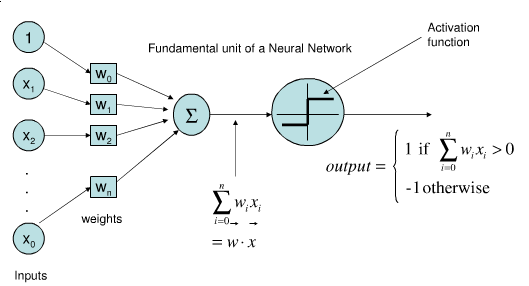
\includegraphics[height=44mm,  width=80mm]{figures/3_nnsingleunit.png}
		\caption[Neural Network - Single Layered Perceptron]{Neural Network - Single Layered Perceptron \footnotemark}
			\label{nnsingleunit}
\end{figure}
\footnotetext{See \url{http://i.stack.imgur.com/KUvpQ.png}}

\subsection{Background}
Historically, the earliest work which laid the foundation of neural networks was done by McCulloch et al.~\parencite{NNFirst:McCull}, which created for the first time, a computational model based on mathematics and algorithms for neural networks. In 1958, Roseblaut F.  ~\parencite{NNFirst:Rose} put forward a pattern recognition algorithm based on a two layer computer learning algorithm. In 1975, Paul Werbos, introduced the back propagation algorithm ~\parencite{NNFirst:Werbos}, which immediately help solved the problem of designing a circuit for the exclusive-or using just perceptron.
\newline

In Artificial Intelligence,  a neural network is modeled either as a function $f:X\rightarrow Y$, or as probability distribution, or inherently defined in form of a learning rule. The simplest one layer neural network is the perceptron. It only has one input layer consisting of neuron inputs $x_i$ and it has one output layer as shown in ~\autoref{nnsingleunit}. First a weighted sum of all the inputs is calculated and then this is later fed to an activation function (Ex. sigmoid, tanh etc.), so as to obtain the output values of these given set of input values within a given range. In the example, the weighted sum is marked as 1, if its positive and greater than 0 and -1 otherwise. Thus, a single layer perceptron works well as a binary classifier. For more complex classification with multiple inputs, one needs a more complex configuration. And also a learning mechanism which can help to send back the intermediate values and learn more accurate weight values. In such cases, hidden layers are introduced comprising purely of neurons, which take the inputs directly and forms an intermediate layer. There can be a number of intermediate layers, but the more the layers, more time it takes to train the machine learning model. The work describes use of one such typical configuration \textit{i.e.,} Feed Forward Neural Networks. Other configurations are recurrent neural network etc. The training is done by using back propagation which is used in tandem with an optimization method, ex. gradient descent. 

\begin{figure}[ht!]
	\centering
		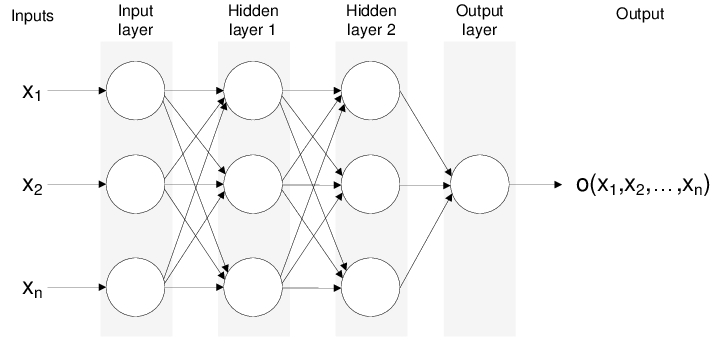
\includegraphics[height=40mm,  width=80mm]{figures/3_multipercep.jpg}
		\caption[Neural Network - Multiple Layered Perceptron]{Neural Network - Multiple Layered Perceptron \footnotemark}
			\label{multipercep}
\end{figure}
\footnotetext{See \url{http://www.intechopen.com/source/html/38302/media/ann.jpg}}

\subsection{Feed Forward Neutral Networks and Back-Propagation}
	Feed forward neural networks \parencite{ffwdnn} are a type of artificial neural network, where the neurons or computation units do not form a cycle. The network proceeds only in one direction. A perceptron is a single layered feed forward neural network, devoid of any hidden layers. The \textit{delta rule} is used in this case for training the perceptron. It calculates the errors and suggests weight adjustment based on difference in output and pre-collected sample output data. This mimics sort of gradient descent algorithm. The output too is in form of a step function, either one value or the other. A multilayer perceptron helps to get more continuous values as output through the use of the activation functions like logistic function. 
 
\begin{center}

$y=\frac{1}{1+e^{x}}$

\end{center}
One such multi-layered perceptron is shown in  ~\autoref{multipercep}. As shown multiple hidden layers are involved between the input and the output layers. It uses back propagation learning algorithm for training. This is performed in two steps: propagation and updating weights. The propagation stage involves starting with a random set of weights and then propagating network forward to get the output activation values. Next we setup the backward propagation where using the sampled target values and the output activation values, we compute the deltas of all output and hidden neurons. This information is used in the next stage of weight update, which computes the weight gradient by multiplying the output delta with input activation. At last, we subtract a ratio of this gradient from the weights and hence learn new weights. The ratio is our learning rate which determines speed and quality of learning. This process is repeated till the network gives sufficient performance. The back propagation algorithm tries to find such set of weights which can minimize the error (in our case the square error E) using gradient descent. As the error needs to be minimized, this can be seen as an optimization problem. Thus, we aim to find first derivative of this error. The error is described as:

\begin{center}
$E=\frac{1}{2} {(t-y)}^2$, where,
\end{center}

E = Squared Error

t = Training Sample's target or expected output

y = Actual computed output of the output neuron.
	

\subsection{Example: Solving Neural Network with Back Propagation}
Consider the following neural network, ~\autoref{nnexample} with given inputs A and B, weights and sigmoid activation function:
$y=\frac{1}{1+e^{-x}}$
\begin{figure}[ht!]
	\centering
		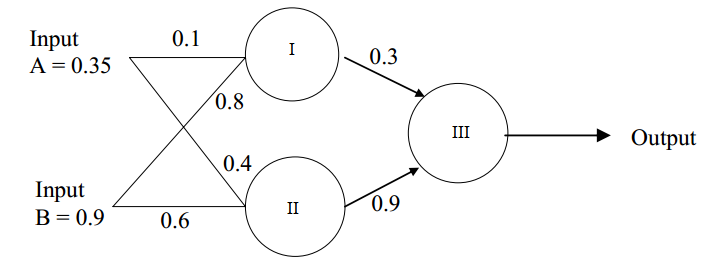
\includegraphics[height=40mm,  width=80mm]{figures/3_nnexample.png}
		\caption[Neural Network - Example]{Neural Network - Example}
			\label{nnexample}
\end{figure}

\textbf{Forward Pass:} Calculating the weighted sum for each neuron.
	
Neuron I : 0.35 $\times$ 0.1 + 0.9 $\times$ 0.8 = 0.755
	
Output I [O(I)]:   $y=\frac{1}{1+e^{-0.755}}$ = 0.68
	
Neuron II: 0.9 $\times$ 0.6 + 0.35 $\times$ 0.4 = 0.68
	
Output II [O(II)]: $y=\frac{1}{1+e^{-0.68}}$ =  0.6637
	
Neuron III: 0.3 $\times$ 0.68 + 0.9 $\times$ 0.6637 = 0.80133
	
Output III [O(III)]: $y=\frac{1}{1+e^{-0.80133}}$ = 0.69
\newline
	
\textbf{Backward Pass:} Original TARGET = 0.5
	
Output Error: $\delta$
	
$\delta$ = (TARGET - O(III)) $\times$ (1-O(III)) $\times$ O(III)

= (0.5-0.69) $\times$ (1-0.69) $\times$ (0.69)
	
= -0.0406
	
New Weights for Output Layer \textit{i.e.}, the weights connecting to Neuron III :
	
For computing the new weights,

${Input_{I}}^+ = Output_{I}$ 
	
${Input_{II}}^+ = Output_{II}$
		
${W_{1}}^+ = {W_{1}} + (\delta \times {Input_{I}}^+ ) $
	
= 0.3 +(-0.0406 $\times$0.68)
	
= 0.2723
	
${W_{2}}^+ = {W_{2}} + (\delta \times{Input_{II}}^+ )$
	
= 0.9 + (-0.0406 $\times$0.6637)
	
= 0.87305
\newline
	
\textbf{Errors for Hidden Layers:}
	
${\delta}_{I} =\delta \times {W}_{1}  \times  (1-O(I))  \times  O(I)$
	
= -0.0406 $\times$ 0.272392 $\times$ (1-0.68) $\times$ 0.68
	
= $-2.406 \times {10}^{-3}$
	
${\delta}_{II} = \delta  \times {W}_{2}  \times (1-O(II)) \times O(II)$
	
= -0.0406 $\times$ 0.87305 $\times$ (1- 0.6637) $\times$ 0.6637
	
= $-7.916 \times {10}^{-3}$
\newline
	
\textbf{New Hidden Layer Weights:}

(Input is A = 0.35 and B = 0.90)
	
${W}_{new} = {W}_{old} + ( \delta   \times Input) $
	
For weights entering Neuron 1:
	
${W_{3}}^+ = 0.1 + (-2.406 \times {10}^{-3}  \times 0.35)$
	
= 0.09916
	
${W_{4}}^+ = 0.8 + (-2.406 \times {10}^{-3}  \times 0.9)$
	
= 0.7978
	
For weights entering Neuron 2:
	
${W_{5}}^+ = 0.4 + (-7.916 \times{10}^{-3}  \times 0.35)$
	
= 0.3972
	
${W_{6}}^+ = 0.6 + (-7.916 \times {10}^{-3}  \times 0.9)$
	
= 0.5928
	

\begin{figure}[ht!]
  \centering
  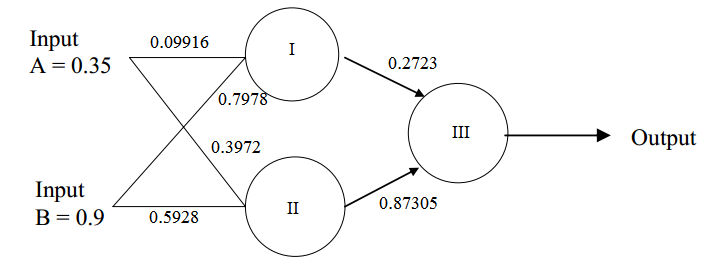
\includegraphics[height=40mm,  width=80mm]{figures/3_nnexample2.png}
  \caption[Neural Network - After one forward and one back propagation step]{Neural Network - After one forward and one back propagation step.}
  \label{nnexample2}
\end{figure}

Thus, after one forward pass and one backward propagation step we have the following neural network as shown in ~\autoref{nnexample2}.
\newline
	
\textbf{Another Forward Pass}

Neuron I: 0.35  $\times$ 0.09916 + 0.9 $\times$ 0.7978 = 0.752726

Output (I): 0.67977  

Neuron II: 0.9 $\times$ 0.5928 + 0.35 $\times$ 0.3972 = 0.67254

Output (II): 0.6620

Neuron III: 0.2723 $\times$ 0.67977 + 0.87305 $\times$ 0.6620 = 0.76306

Output (III): 0.68201
\newline

\textbf{Computing Overall Error:}

${Target}_{Original}$ = 0.50

${Target}_{Pass 1}$ = 0.69

Error (Pass 1) = ${Target}_{Original} - {Target}_{Pass 1}$

= - 0.19

${Target}_{Original}$ = 0.50

${Target}_{Pass 2}$ = 0.68201

Error (Pass 2) = ${Target}_{Original} - {Target}_{Pass 2}$

= - 0.18201
\newline

So, we find: \textbf{Error (Pass 2)  is less than Error (Pass 1)} Therefore, the error has reduced.
\newline 

We repeat this process, till the point that, we have no reduction in overall error. At each iteration, the machine automatically adjusts it's internal parameters or weights, which cause the error to be reduced. At this point the process is stopped and the learned weights are chosen as our final weights. These weights can be used to a random input to predict the correct class or output.

\section{From Neural Networks to Deep Neural Networks}
In subsection 3.1.3, we saw a simple two unit, single hidden layer neural network and its working through back-propagation algorithm. We was the most important take away message is the most important outcome of this learning procedure is actually to \textbf{learn the correct weights} for the network. We saw that to properly compute weights, the algorithm computes a gradient vector that, for each weight, indicates by what amount the error would increase or decrease if the weight were increased by a tiny amount. The weight vector is then adjusted in the opposite direction to the gradient vector. This negative value of the gradient vector takes the objective function (averaged over all training values in a high dimensional plane of weight vectors) to its minimum value, where the output error is low on average.

The commonly used procedure to achieve this is\textbf{ Stochastic Gradient Descent }(SGD). This consists of showing the input vector for a few examples, computing the outputs and the errors, computing the average gradient for those examples, and adjusting the weights accordingly. The process is repeated for many small sets of examples from the training set until the average of the objective function stops decreasing. It is called \textit{stochastic} because each small set of examples gives a noisy estimate of the average gradient over all examples.~\parencite{naturearticle} This is highly efficient technique as compared to other optimization techniques. Later, the system's performance is evaluated over a test set. this is a good generalization of the trained model since it helps us to test model on unseen data. 
\newline

Most current systems based on machine learning use the two class classifier over hand crafted features. although, these are effective to an extent, but they do not fully understand the underlying complexity. For making the classifiers more powerful towards the given task, one can use the non-linear features as used in Kernel Methods ~\parencite{learnkernels}, but even the features which arise with traditional Gaussian Kernels, do not generalize well far from the examples seen during training. The alternative is to hand craft features, but as we know its a tedious task. The better way as we know it is to learn features automatically. This is an advantage of Deep Learning.
\newline

A \textbf{deep learning architecture} can be visualized as a \textbf{multi-layered stack} of simple modules of learning which are responsible to compute \textbf{non-linear input-output mappings}. Each module aims to transform the input to increase both the selectivity and in-variance of the representation. The system can implement many complex and intricate functions if we increase the number of such non-linear layers (to a depth of 5 - 20) and model relevant parts of the input and also leave out irrelevant details, leading to a more concise and precise representation.    

\begin{figure}[ht!]
  \centering
  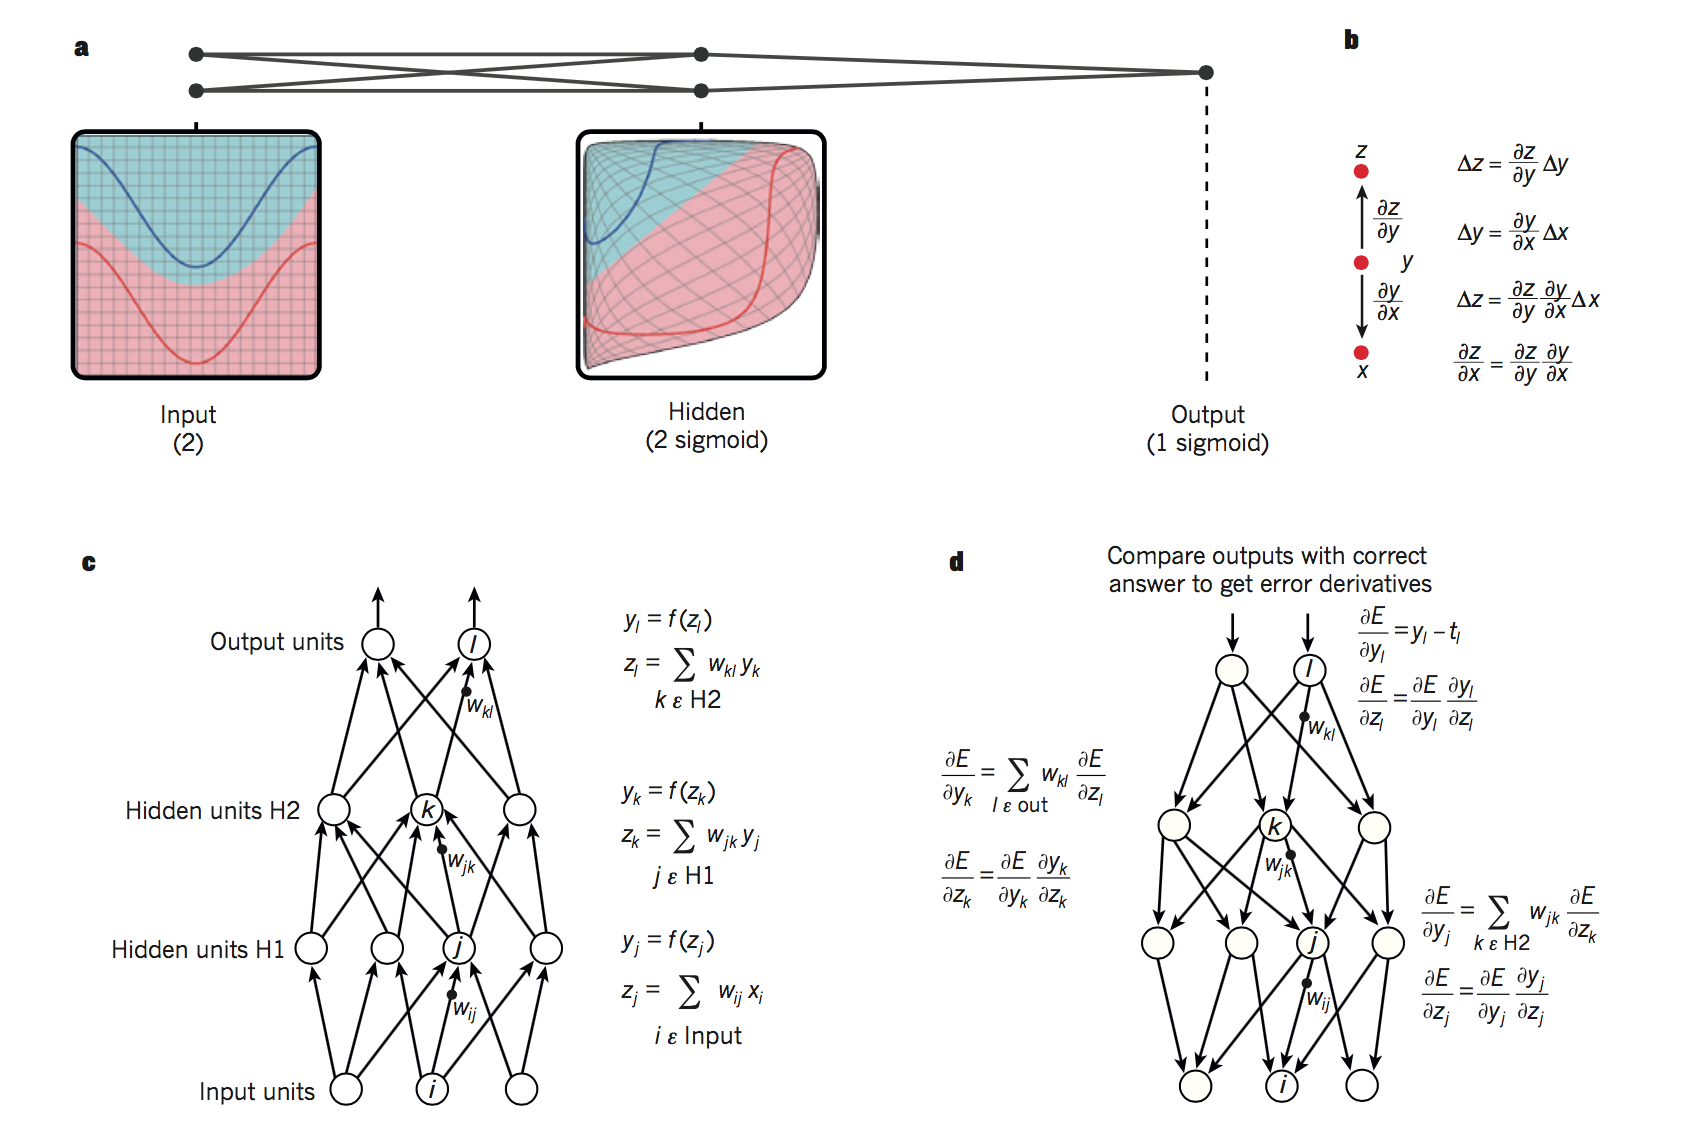
\includegraphics[height=130mm,  width=160mm]{figures/3_nnbackprop.png}
  \caption[Multi-layered Neural Networks and Back-Propagation]{Multi-layered Neural Networks and Back-Propagation \footnotemark}
  \label{nnbackpropex}
\end{figure}
 \footnotetext{See \url{http://colah.github.io/}}

Many Deep Learning Applications use Feed forward Neural Network Architectures ~\autoref{nnbackpropex}., which learn to map fixed sized input to a fixed sized output. to go from one layer to the next, a set of units compute a weighted sum of their inputs from the previous layers and pass the result through a non linear function. In the past, traditional neural networks used the \textbf{sigmoid} or \textbf{hyperbolic tangent} non linear functions. The more recent deep learning architectures rely of \textbf{rectified linear units }(ReLU). They are otherwise known as half wave rectifiers f(z) = max(z,0). They are exceptionally good at learning at a much faster rate in multi-layered networks and allow training of a deep supervised network without unsupervised pre-training. The hidden units in the hidden layer (layers other than the input and output layer) distort the input signal in a non linear way such that the categories become separable by the last layer.
\newline

Also, if we look at the history of neural networks, they started out brilliantly in solving a number of AI problems and showing good results, but by late 1990's they weren't as highly regarded. One of the main proponents against their adoption was the underlying use of Stochastic Gradient Descent. It was thought that while exploring the global minimum value for the objective function, the method might get to only the \textbf{local minima}. Thus the weight configuration changes were not considered  highly optimized. What was found later in practice with large multi-layered networks working on high dimensions is that this problem has hardly any significant effect. In fact, the results using a local minima or a global minima are often quite comparable.
\newline 

In 2006, the research group from Canada Institute for Advanced Research (CIFAR),   introduced unsupervised learning methods that created layers of feature detectors using unlabeled input data. The objective in learning, each layer was to model the activities of layers below it. Using a reconstruction objective and pre-training several layers of  complex feature detectors, the weights of neural network can be initialized to proper values.  A final layer is later added to the system and the system itself is then fine tuned using back-propagation. This was a huge breakthrough as it worked remarkably well for recognizing hand written digits or for detecting pedestrians, even though the amount of hand labeled data was limited.
\newline

Later this pretraining approach, helped in speech recognition, partly with the adoption and ease of use of Graphical Processing Units (GPU), which allowed a 10x - 20x times of increase in overall training time. the procedure was able to beat the current state of the art with ease and by 2012, the method was fine tuned and adopted into mobile hand held devices running Android\footnotemark. 
Interestingly, it was found out through numerous experiments that pre-training is useful for the case where we have a small data-set to begin with. Another class of deep feed forward neural network which have gained popularity are the \textbf{Convolutional Neural Networks} (CNN). They are easiest to train and generalize much better than the networks which had full connectivity between the layers. These have been remarkable in several image processing tasks and have been adopted widely by the computer vision community. 